\documentclass[aspectratio=169,10pt]{beamer}

% ============================================================
% SmartBite - Phase-II PBL Evaluation
% Based on the provided Graphic Era Phase-II template
% ============================================================
\usepackage[T1]{fontenc}
\usepackage[utf8]{inputenc}
\usepackage{graphicx}
\usepackage{tikz}
\usetikzlibrary{positioning,arrows.meta}
\usepackage{xcolor}
\usepackage{booktabs}
\usepackage{tabularx}
\usepackage{array}
\usepackage{ragged2e}
\usepackage{hyperref}

\definecolor{GEUBlue}{RGB}{20,55,105}
\definecolor{GEULightBlue}{RGB}{238,244,251}
\definecolor{GEUGrey}{RGB}{90,90,90}
\definecolor{GEULightGrey}{RGB}{245,246,248}

\usetheme{default}
\setbeamertemplate{navigation symbols}{}
\setbeamertemplate{blocks}[rounded][shadow=false]
\setbeamercolor{normal text}{fg=black,bg=white}
\setbeamercolor{frametitle}{fg=GEUBlue}
\setbeamercolor{structure}{fg=GEUBlue}
\setbeamercolor{block title}{fg=GEUBlue,bg=GEULightBlue}
\setbeamercolor{block body}{fg=black,bg=GEULightBlue}
\setbeamerfont{frametitle}{size=\Large,series=\bfseries}

% Add graphicera_logo.png to the same Overleaf project if available.
\newcommand{\GEULogo}{graphicera_logo.png}
\newcommand{\smallnote}[1]{\vspace{0.08cm}{\scriptsize\color{GEUGrey}#1}}
\newcommand{\placeholder}[1]{\textit{\color{GEUGrey}#1}}

% Header: display the logo only when the image file exists.
\setbeamertemplate{headline}{%
  \begin{tikzpicture}[remember picture,overlay]
    \IfFileExists{\GEULogo}{
      \node[anchor=north east,xshift=-0.30cm,yshift=-0.12cm]
      at (current page.north east)
      {\includegraphics[height=0.62cm]{\GEULogo}};
    }{}
  \end{tikzpicture}
  \vspace{0.72cm}
}
\setbeamertemplate{frametitle}{%
  \vspace{0.03cm}\insertframetitle\par
  \vspace{0.04cm}\textcolor{GEUBlue}{\rule{\textwidth}{0.9pt}}
  \vspace{0.03cm}
}
\setbeamertemplate{footline}{%
  \leavevmode
  \hbox{%
    \begin{beamercolorbox}[wd=.82\paperwidth,ht=0.32cm,dp=0.10cm,leftskip=.3cm]{author in head/foot}
      \tiny Department of Computer Science \& Engineering | Graphic Era (Deemed to be University)
    \end{beamercolorbox}%
    \begin{beamercolorbox}[wd=.18\paperwidth,ht=0.32cm,dp=0.10cm,rightskip=.3cm]{date in head/foot}
      \hfill\tiny\insertframenumber/\inserttotalframenumber
    \end{beamercolorbox}}
}

\title{\textbf{Project-Based Learning}\\[2mm]\large Phase-II Evaluation}
\author{\textbf{SmartBite: Intelligent Food Recommendation \& Route Optimization System}\\Team ID: {DSCPP-III-2026-T076}}
\institute{Department of Computer Science \& Engineering\\Graphic Era (Deemed to be University), Dehradun}
\date{Academic Session 2026--27}

\begin{document}









% SLIDE 1
\begin{frame}[plain]
\begin{tikzpicture}[remember picture,overlay]
  \draw[GEUBlue,line width=3pt] (current page.north west)--(current page.north east);
  \IfFileExists{\GEULogo}{
    \node[anchor=north east,xshift=-0.45cm,yshift=-0.35cm] at (current page.north east)
    {\includegraphics[height=1.0cm]{\GEULogo}};
  }{}
  \node[align=center,text width=.86\paperwidth] at ([yshift=.25cm]current page.center) {
    {\color{GEUBlue}\fontsize{26}{30}\selectfont\bfseries PROJECT-BASED LEARNING}\\[3mm]
    {\fontsize{18}{22}\selectfont PHASE-II EVALUATION}\\[7mm]
    {\color{GEUGrey}\Large\bfseries SmartBite: Intelligent Food Recommendation\\ \& Route Optimization System}\\[3mm]
    {\color{GEUBlue}\normalsize Team ID: DSCPP-III-2026-T076}
  };
  \node[align=center,anchor=south,yshift=.42cm] at (current page.south) {
    \bfseries Department of Computer Science \& Engineering\\
    Graphic Era (Deemed to be University), Dehradun\\[-1mm]
    \scriptsize Academic Session 2026--27
  };
\end{tikzpicture}
\end{frame}














% SLIDE 2
\begin{frame}{Team \& Mentor Details}
\begin{columns}[T,totalwidth=\textwidth]
\column{.48\textwidth}
\begin{block}{Team Information}
\begin{tabular}{@{}ll@{}}
\textbf{Team ID:} & DSCPP-III-2026-T076\\
\textbf{Semester:} & 3rd\\

\textbf{Domain:} & Food recommendation \& routing
\end{tabular}
\end{block}
\column{.48\textwidth}
\begin{block}{Team Members}
1. Dhairya Bhardwaj -- 2510012362\\[2mm]
2. Devvrat Sharma -- 2510012427\\[2mm]
3. Komal Singh -- 2510360150\\[2mm]
4. Nimish Sharma -- 2510360065
\end{block}
\end{columns}
\vspace{2mm}
\begin{block}{Mentor}
Mr. Upendra Aswal\hfill
\textbf{Interactions completed:} Not specified
\end{block}

\end{frame}
















% SLIDE 3
\begin{frame}{Phase-I Recap \& Phase-II Progress}
\begin{block}{Phase-I Recap}
SmartBite is designed to help users explore food options by selecting a location and cuisine, viewing restaurant and menu information, and considering road-distance information when choosing a restaurant.
\end{block}
\begin{columns}[T,totalwidth=\textwidth]
\column{.48\textwidth}
\textbf{\color{GEUBlue}Phase-I Baseline}
\begin{itemize}\itemsep3pt
\item Problem statement and objectives established.
\item Four major implementation areas identified.
\item Phase-II focuses on implementation and validation.
\end{itemize}
\column{.48\textwidth}
\textbf{\color{GEUBlue}Phase-II Development}
\begin{itemize}\itemsep3pt
\item Separated the implementation into Data, Graph, Dining, and Registration modules.
\item Added structured restaurant, cuisine, dish, menu, location, and road data.
\item Developed registration/login and password creation/checking functions.
\end{itemize}
\end{columns}

\end{frame}
















% SLIDE 4
\begin{frame}{Problem Statement \& Finalized Objectives}
\begin{block}{Problem Statement}
Finding a suitable restaurant can require users to compare location, cuisine, restaurant information, menu choices, and travel distance. SmartBite organizes this information in one C++ application and uses road-graph data to support distance-based restaurant selection.
\end{block}
\textbf{\color{GEUBlue}Objectives}
\begin{enumerate}\itemsep2pt
\item Maintain structured information about locations, restaurants, cuisines, dishes, menus, and roads.
\item Allow users to register or log in and select the service they want to use.
\item Filter and display restaurants based on user selections such as location and cuisine.
\item Represent road connections as a graph and calculate shortest distances where implemented.
\end{enumerate}

\end{frame}

















% SLIDE 5
\begin{frame}{Updated System Architecture / Workflow}
\begin{center}
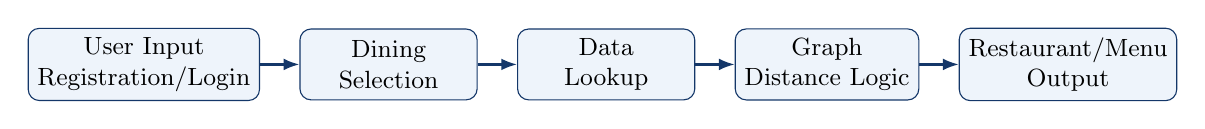
\begin{tikzpicture}[
node distance=5mm,
box/.style={rectangle,rounded corners,draw=GEUBlue,fill=GEULightBlue,minimum width=2.25cm,minimum height=9mm,align=center,font=\small},
arrow/.style={-{Latex[length=2mm]},thick,draw=GEUBlue}
]
\node[box] (user) {User Input\\Registration/Login};
\node[box,right=of user] (dining) {Dining\\Selection};
\node[box,right=of dining] (data) {Data\\Lookup};
\node[box,right=of data] (graph) {Graph\\Distance Logic};
\node[box,right=of graph] (out) {Restaurant/Menu\\Output};
\draw[arrow] (user)--(dining);
\draw[arrow] (dining)--(data);
\draw[arrow] (data)--(graph);
\draw[arrow] (graph)--(out);
\end{tikzpicture}
\end{center}
\vspace{3mm}
\begin{columns}[T,totalwidth=\textwidth]
\column{.48\textwidth}
\textbf{\color{GEUBlue}Major Components}
\begin{itemize}\itemsep2pt
\item Registration and password module
\item Data lookup module
\item Graph and route-distance module
\item Dining workflow and results
\end{itemize}
\column{.48\textwidth}
\textbf{\color{GEUBlue}Data Flow}
\begin{itemize}\itemsep2pt
\item User provides account and dining choices.
\item Dining uses Data functions to retrieve information.
\item Graph logic evaluates road connections and distance.
\item The application displays relevant restaurant/menu details.
\end{itemize}
\end{columns}

\end{frame}



















% SLIDE 6
\begin{frame}{Module Design \& Functional Requirements}
\small
\begin{columns}[T,totalwidth=\textwidth]
\column{.48\textwidth}
\textbf{\color{GEUBlue}Major Modules}
\begin{enumerate}\itemsep4pt
\item \textbf{Registration:} register/login, username checking, password generation and strength checking.
\item \textbf{Data:} location, restaurant, cuisine, dish, menu, and road information.
\item \textbf{Graph:} adjacency-list representation of road connections and shortest-distance logic.
\item \textbf{Dining:} user selections, restaurant filtering, restaurant details, and menu display.
\end{enumerate}
\column{.48\textwidth}
\textbf{\color{GEUBlue}Functional Requirements}
\begin{itemize}\itemsep4pt
\item Validate usernames and support account access.
\item Retrieve relevant restaurant and menu records.
\item Represent connections between locations.
\item Present dining options based on selected criteria.
\end{itemize}
\end{columns}

\end{frame}


















% SLIDE 7
\begin{frame}{Technology Stack \& Development Methodology}
\begin{columns}[T,totalwidth=\textwidth]
\column{.48\textwidth}
\begin{block}{Technology Stack}
\begin{itemize}\itemsep3pt
\item Programming language: C++
\item Data structures: vectors, strings, adjacency lists
\item Algorithm: Dijkstra's shortest-path algorithm (where implemented)
\item Development environment: Visual Studio Code with C++ compiler
\item Version control: Git and GitHub, if used for this project
\end{itemize}
\end{block}
\column{.48\textwidth}
\begin{block}{Development Methodology}
\begin{enumerate}\itemsep3pt
\item Requirement analysis
\item Module design
\item Independent module development
\item Integration of module calls
\item Testing and validation
\end{enumerate}
\end{block}
\end{columns}

\end{frame}




















% SLIDE 8
\begin{frame}{Implementation of PBL Course Concepts}
\scriptsize
\begin{center}
\renewcommand{\arraystretch}{1.35}
\begin{tabularx}{.96\textwidth}{@{}>{\bfseries}p{3.0cm}X p{2.5cm}@{}}
\toprule
Course / Area & Concepts implemented in SmartBite & Project module\\
\midrule
Data Structures & Graph adjacency list, vectors/collections, structured records and lookup operations & Data, Graph, Dining\\
OOP with C++ & User class, objects, encapsulation, constructors, strings and vectors & Registration\\
Algorithms & Shortest-distance calculation using Dijkstra's algorithm, if enabled in current build & Graph, Dining\\
Modular Programming & Functions separated by responsibility and called through module workflows & All modules\\
\bottomrule
\end{tabularx}
\end{center}
\vspace{4mm}
\begin{block}{Important}
Demonstrate each listed concept from the current code during evaluation.
\end{block}
\end{frame}



















% SLIDE 9
\begin{frame}{Development \& Implementation Progress}
\scriptsize
\begin{center}
\renewcommand{\arraystretch}{1.35}
\begin{tabularx}{.96\textwidth}{@{}p{2.5cm}p{2.3cm}X@{}}
\toprule
\textbf{Module} & \textbf{Status} & \textbf{Known implementation scope}\\
\midrule
Registration \& Password & Implemented; integration check required & Registration/login flow, username check, manual/automatic password creation, password strength checking, service selection\\
Data & Implemented; integration check required & Location, restaurant, cuisine, dish, menu, and road data with lookup/filter functions\\
Graph & Integration check required & Graph representation, road connections, shortest-distance calculation\\
Dining & Implemented; integration check required & Location/cuisine selection, restaurant filtering/details, menu display, and use of distance information\\
\bottomrule
\end{tabularx}
\end{center}
\vspace{4mm}
\begin{block}{Overall Completion}
Final integrated completion: pending verification.
\end{block}

\end{frame}




















% SLIDE 10
\begin{frame}{Working Prototype / Demonstration}
\begin{columns}[T,totalwidth=\textwidth]
\column{.45\textwidth}
\textbf{\color{GEUBlue}Features to Demonstrate}
\begin{itemize}\itemsep4pt
\item Register/login and password options
\item Select a location and cuisine
\item View matching restaurants and menu details
\item Show road-distance/shortest-path output, if working in the integrated build
\end{itemize}
\column{.51\textwidth}
\begin{block}{Prototype / Output Evidence}
\centering
\vspace{5mm}
Console output screenshot to be added\\[4mm]
Route output screenshot: add only if verified
\vspace{5mm}
\end{block}
\end{columns}

\end{frame}
















% SLIDE 11
\begin{frame}{Testing Plan \& Validation}
\scriptsize
\begin{center}
\renewcommand{\arraystretch}{1.35}
\begin{tabularx}{.96\textwidth}{@{}p{2.2cm}X X p{1.3cm}@{}}
\toprule
Test / Module & Expected result & Current record & Status\\
\midrule
Registration & New username is accepted; duplicate username is handled & Not recorded yet & Not tested\\
Dining filter & Selected location/cuisine returns matching restaurant records & Not recorded yet & Not tested\\
Graph distance & Shortest-distance result matches a manually checked route & Not recorded yet & Not tested\\
Menu lookup & Selected restaurant displays its associated menu information & Not recorded yet & Not tested\\
\bottomrule
\end{tabularx}
\end{center}
\vspace{3mm}
\begin{block}{Validation}
Run each test on the integrated build and record the observed result. Do not present unexecuted tests as passed.
\end{block}
\end{frame}



















% SLIDE 12
\begin{frame}{GitHub Repository \& Development Activity}
\begin{columns}[T,totalwidth=\textwidth]
\column{.46\textwidth}
\textbf{\color{GEUBlue}Repository Information}
\begin{itemize}\itemsep4pt
\item Repository: show the verified team repository during the demo
\item README: setup and usage instructions
\item Contributors: verify team access
\item Repository status: latest code to be confirmed
\item Branches: show if applicable
\end{itemize}
\column{.50\textwidth}
\textbf{\color{GEUBlue}Development Activity}
\begin{itemize}\itemsep4pt
\item Record commits for module development.
\item Use meaningful commit messages.
\item Ensure individual contributions are visible.
\item Upload the latest working implementation.
\item Keep setup and usage instructions in the README.
\end{itemize}
\end{columns}

\end{frame}

















% SLIDE 13
\begin{frame}{Individual Contribution}
\scriptsize
\begin{center}
\renewcommand{\arraystretch}{1.4}
\begin{tabularx}{.96\textwidth}{@{}p{2.0cm}p{2.0cm}X p{1.6cm}@{}}
\toprule
Member & Role & Technical contribution & Commits\\
\midrule
Dhairya & Team Lead & Dine-in module & Check Git history\\
Devvrat & Member & Delivery module & Check Git history\\
Komal & Member & Login, password and feedback modules & Check Git history\\
Nimish & Member & Takeaway and drive-through module & Check Git history\\
\bottomrule
\end{tabularx}
\end{center}
\vspace{3mm}
\begin{block}{Individual Evaluation}
Each member should explain their own contribution and verify commit counts from Git history.
\end{block}
\end{frame}
















% SLIDE 14
\begin{frame}{Challenges, Remaining Work \& Phase-III Roadmap}
\begin{columns}[T,totalwidth=\textwidth]
\column{.48\textwidth}
\textbf{\color{GEUBlue}Integration Risks to Check}
\begin{itemize}\itemsep3pt
\item Keeping module interfaces consistent during integration.
\item Ensuring restaurant, location, and road data use consistent identifiers.
\item Validating shortest-path results and edge cases.
\end{itemize}
\vspace{2mm}
\textbf{\color{GEUBlue}Solutions / Learning}
\begin{itemize}\itemsep3pt
\item Use clearly separated functions and shared data conventions.
\item Test each module independently before integrated testing.
\end{itemize}
\column{.48\textwidth}
\textbf{\color{GEUBlue}Phase-III Roadmap}
\begin{enumerate}\itemsep4pt
\item Verify and complete remaining module functions.
\item Finish end-to-end integration.
\item Run positive, negative, and edge-case tests.
\item Improve recommendation and distance handling.
\item Complete documentation and final demonstration.
\end{enumerate}
\end{columns}

\end{frame}



















% SLIDE 15
\begin{frame}{Expected Outcomes \& References}
\begin{columns}[T,totalwidth=\textwidth]
\column{.47\textwidth}
\textbf{\color{GEUBlue}Expected Final Outcomes}
\begin{itemize}\itemsep3pt
\item An integrated SmartBite prototype.
\item Structured restaurant and menu information.
\item Location/cuisine-based restaurant browsing.
\item Road-distance support for restaurant selection.
\item Registration and password-handling workflow.
\end{itemize}
\column{.47\textwidth}
\textbf{\color{GEUBlue}References}
\begin{enumerate}\itemsep3pt
\item B. Stroustrup, \textit{The C++ Programming Language}.
\item Cormen et al., \textit{Introduction to Algorithms}.
\item E. W. Dijkstra, ``A Note on Two Problems Connected with Graphs,'' 1959.
\item C++ Standard Library documentation.
\end{enumerate}
\vfill
\begin{center}
\colorbox{GEUBlue}{\parbox{.78\textwidth}{\centering\color{white}\textbf{Thank You}\\Questions \& Suggestions}}
\end{center}
\end{columns}

\end{frame}

\end{document}
